\reading{MR-3}{Parametric Approaches (II): Extreme Value}{strike}{5}
% ==========================================================

\begin{mrkeybox}[title={Learning objectives in this reading}]
\small
\begin{enumerate}[label=\textbf{\alph*.},leftmargin=1.7em]
\item Explain the importance and challenges of extreme values in risk management.
\item Describe extreme value theory (EVT) and its use in risk management.
\item Describe the peaks-over-threshold (POT) approach.
\item Compare and contrast the generalized extreme value (GEV) and POT approaches to estimating
      extreme risks.
\item Discuss the application of the generalized Pareto (GP) distribution in the POT approach.
\item Explain the multivariate EVT for risk management.
\end{enumerate}
\end{mrkeybox}

% ---------------------------------------------------------
\lo{MR-3 a}{Explain the importance and challenges of extreme values in risk management.}

\begin{mrdefbox}[title={Extreme values}]
Extreme events are low-probability, high-impact events that can be very costly. Rare extreme
events --- market crashes, crises, catastrophes --- are infrequent but highly impactful, and
they can lead to substantial financial losses, which makes their identification and management
crucial.
\end{mrdefbox}

\subsection{Why it is a problem}
\begin{itemize}
\item The estimation of extreme risks poses a difficult problem due to the rarity of these
      events and the limited number of extreme observations available.
\item They can have significant financial consequences.
\end{itemize}

\subsection{Examples of extreme events}
Unprecedented stock market falls, the failures of major institutions, the outbreak of financial
crises, and natural catastrophes.

\subsection{Challenges}
\begin{itemize}
\item Limited data for modeling extreme events. Estimating risks associated with extreme events
      is challenging due to their rarity.
\item Unobserved extreme scenarios pose a challenge. Estimates of extreme risks must therefore
      be very uncertain, and this uncertainty is especially pronounced if we are interested in
      extreme risks not only within the range of observed data, but well beyond it.
\item Distribution assumptions may not precisely match reality, introducing errors.
\item Overreliance on central tendency measures can miss the extreme value issue.
\end{itemize}

\subsection{Approaches to address the challenges}
\begin{itemize}
\item Develop specialized estimation methods for extreme values.
\item Learn from other fields (e.g.\ flood control) facing similar problems in estimating
      extremes beyond historical data.
\end{itemize}

% ---------------------------------------------------------
\lo{MR-3 b}{Describe extreme value theory (EVT) and its use in risk management.}

Extreme-value theory (EVT), which is what this entire chapter is about, is a branch of applied
statistics tailored to estimating risks associated with extreme events, which are rare but
potentially highly impactful occurrences.

EVT differs from traditional central tendency statistics as it focuses on extreme values rather
than averages. Extreme-value distributions and their parameters are distinct from central
tendency statistics, making parameter estimation more difficult. EVT uses extreme-value theorems
to select suitable distributions and estimate parameters for extreme data.

\begin{mrkeybox}[title={The EVT process}]
\begin{enumerate}[label=\textbf{\alph*.}]
\item In the first step of EVT, a large sample is taken from an unknown distribution.
\item The maximum value within this sample is determined, and is considered an extreme value.
\item As the sample size increases, the distribution of these extreme values converges towards
      the generalized extreme value (GEV) distribution.
\end{enumerate}
\end{mrkeybox}

\subsection{Fisher-Tippett theorem}
One approach for estimating parameters is the Fisher-Tippett theorem. According to this theorem,
as the sample size $n$ gets large, the distribution of extremes, denoted $M_n$, converges to the
following distribution known as the generalized extreme value (GEV) distribution.

\begin{mrfmlbox}
\begin{align*}
F(X \mid \xi, \mu, \sigma) &= \exp\!\left[ -\left( 1 + \xi \times \frac{x-\mu}{\sigma}
   \right)^{\!-1/\xi} \right] && \text{if } \xi \neq 0\\[4pt]
F(X \mid \xi, \mu, \sigma) &= \exp\!\left[ -\exp\!\left( \frac{x-\mu}{\sigma} \right) \right]
   && \text{if } \xi = 0
\end{align*}
\mrvk{$x$ = the extreme value being evaluated;\quad $\mu$ = the \textit{location} parameter;\quad
$\sigma$ = the \textit{scale} parameter;\quad $\xi$ = the \textit{tail index}, which sets the
shape of the tail.}{}
\end{mrfmlbox}

\begin{mrkeybox}[title={Note on the parameters}]
The parameters $\mu$ and $\sigma$ are the location parameter and scale parameter respectively.
Although related to the mean and variance, they are \textit{not} the same; they serve the same
purpose in extreme-value analysis. The symbol $\xi$ is the tail index and indicates the shape
(or heaviness) of the tail of the limiting distribution. It defines the type of GEV
distribution.
\end{mrkeybox}

\subsection{The three cases of the GEV distribution}

\begin{center}
\small
\begin{tabularx}{\linewidth}{@{}p{1.7cm} p{2.7cm} p{2.1cm} >{\raggedright\arraybackslash}X@{}}
\arrayrulecolor{FRMRule}\toprule
\rowcolor{FRMNavy} \hdr{Tail index} & \hdr{GEV becomes} & \hdr{Tails are} & \hdr{Typical parent distributions}\\
\midrule
$\xi > 0$ & \textbf{Frechet} & ``Heavy'' & $t$-distribution and Pareto distributions\\
\rowcolor{FRMSoft}
$\xi = 0$ & \textbf{Gumbel} & ``Light'' & Normal and lognormal distributions\\
$\xi < 0$ & \textbf{Weibull} & ``Lighter'' than a normal distribution & Rare in financial models\\
\bottomrule
\end{tabularx}
\end{center}
\figcap{Distributions where $\xi < 0$ do not often appear in financial models; therefore,
financial risk management analysis can essentially focus on the first two cases, $\xi > 0$ and
$\xi = 0$.}

\begin{center}
\begin{tikzpicture}
\begin{axis}[
  width=11.0cm, height=5.4cm,
  xmin=-1.8, xmax=6.5, ymin=0, ymax=0.45,
  xlabel={\scriptsize Extreme value $x$},
  ylabel={\scriptsize Density},
  xlabel style={font=\scriptsize}, ylabel style={font=\scriptsize},
  tick label style={font=\scriptsize},
  xtick={-1,0,1,2,3,4,5,6}, ytick={0,0.1,0.2,0.3,0.4},
  legend style={font=\scriptsize\sffamily, draw=FRMRule, fill=white,
    at={(0.5,-0.30)}, anchor=north, legend columns=-1, column sep=8pt},
  axis line style={draw=black!55}, clip=false]
\addplot[FRMRed, line width=1.3pt, smooth, domain=-1.85:6.5, samples=180]
  {((1+0.5*x)^(-2))^(1.5)*exp(-((1+0.5*x)^(-2)))};
\addlegendentry{$\xi > 0$ --- Frechet, \textbf{heavy}}
\addplot[FRMNavy, line width=1.3pt, dashed, smooth, domain=-1.8:6.5, samples=180]
  {exp(-x)*exp(-exp(-x))};
\addlegendentry{$\xi = 0$ --- Gumbel, \textbf{light}}
\addplot[FRMGreen, line width=1.3pt, dotted, smooth, domain=-1.8:1.98, samples=180]
  {((1-0.5*x)^(2))^(0.5)*exp(-((1-0.5*x)^(2)))};
\addlegendentry{$\xi < 0$ --- Weibull, \textbf{lighter, bounded}}
\draw[FRMGreen!60, dashed, line width=0.7pt] (axis cs:2,0) -- (axis cs:2,0.10);
\node[anchor=west, font=\tiny\sffamily, text=FRMGreen, fill=white, inner sep=1.2pt,
  align=left] at (axis cs:2.15,0.155) {Weibull \textbf{stops} here:\\ finite upper bound};
\node[anchor=west, font=\tiny\sffamily, text=FRMRed, fill=white, inner sep=1.2pt]
  at (axis cs:3.9,0.055) {Frechet tail still alive out here};
\end{axis}
\end{tikzpicture}
\end{center}
\figcap{The tail index is not an abstract parameter --- it \textit{is} the tail. At
$\xi < 0$ the distribution has a finite upper bound and simply stops, which is why it is no use
for financial losses. At $\xi = 0$ the tail decays exponentially. At $\xi > 0$ it decays as a
power, so extreme values remain possible far out. Everything in the table above is this one
picture read three ways.}

\subsection{So how do we select between Frechet and Gumbel?}
\begin{enumerate}
\item \term{Confidence in the parent distribution.} If the researcher is confident about a
      specific distribution --- a $t$-distribution, for example --- then the researcher should
      assume $\xi > 0$.
\item \term{Statistical testing.} The researcher applies a statistical test and cannot reject
      the hypothesis $\xi = 0$. In this case, the researcher uses the assumption $\xi = 0$.
\item \term{Conservatism.} Given the dangers of model risk, and bearing in mind that the
      estimated risk measure increases with the tail index, a safer option is always to choose
      the Fr\'echet. The researcher may wish to be conservative and assume $\xi > 0$ to avoid
      model risk.
\end{enumerate}

% ---------------------------------------------------------
\lo{MR-3 c}{Describe the peaks-over-threshold (POT) approach.}

\begin{mrdefbox}[title={Peaks-over-threshold (POT)}]
\begin{enumerate}[label=\textbf{\alph*.}]
\item The peaks-over-threshold (POT) approach is an application of extreme value theory to the
      distribution of excess losses over a high threshold, $u$.
\item The POT approach generally requires \term{fewer parameters} than approaches based on
      extreme value theorems. The POT approach provides the natural way to model values that
      are greater than a high threshold, and in this way it corresponds to the GEV theory by
      modeling the maxima or minima of a large sample.
\item It assumes that observations beyond the threshold follow a \term{generalized Pareto
      distribution} whose parameters can be estimated.
\end{enumerate}
\end{mrdefbox}

We define $u$ as the threshold value for positive values of $x$, and the distribution of excess
losses over our threshold $u$ as:

\begin{mrfmlbox}
\[ F_u(x) \;=\; P\{X - u \le x \mid X > u\} \;=\; \frac{F(x+u) - F(u)}{1 - F(u)} \]
\mrvk{$u$ = the chosen high threshold;\quad $x$ = the size of the excess above that threshold;\quad
$F(\cdot)$ = the cumulative distribution function of the underlying losses;\quad $F_u(x)$ = the
distribution of the excess, conditional on the threshold having been breached.}{}
\end{mrfmlbox}

This is the conditional distribution for $X$ given that the threshold is exceeded by no more
than $x$.

\begin{center}
\begin{tikzpicture}
\begin{axis}[
  width=10.4cm, height=4.6cm,
  xmin=-4.2, xmax=4.6, ymin=0, ymax=0.46,
  axis y line=none, axis x line=bottom, axis line style={draw=black!55},
  tick label style={font=\scriptsize}, xtick={\empty},
  clip=false]
\addplot[domain=-4:4.4, samples=200, smooth, black!80, line width=0.9pt] {0.39894*exp(-x^2/2)};
\addplot[domain=1.6:4.4, samples=120, smooth, draw=none, fill=FRMRed!35] {0.39894*exp(-x^2/2)}
  \closedcycle;
\draw[FRMNavy, dashed, line width=0.8pt] (axis cs:1.6,0) -- (axis cs:1.6,0.30);
\node[anchor=south, font=\scriptsize\sffamily, text=FRMNavy] at (axis cs:1.6,0.31)
  {threshold $u$};
\draw[FRMRed, {Stealth[length=4pt]}-{Stealth[length=4pt]}, line width=0.6pt]
  (axis cs:1.7,0.055) -- (axis cs:4.3,0.055);
\node[anchor=south, font=\scriptsize\sffamily, text=FRMRed] at (axis cs:3.0,0.06)
  {excess losses, $x$};
\node[anchor=north, font=\scriptsize\sffamily, text=black!60] at (axis cs:-1.2,-0.01)
  {body of the distribution --- ignored by POT};
\end{axis}
\end{tikzpicture}
\end{center}
\figcap{POT throws away the body of the loss distribution entirely and models only what lies
beyond the threshold $u$. The quantity being modelled is the \textit{excess} $x$, measured from
$u$ upward, not the loss itself.}

\begin{center}
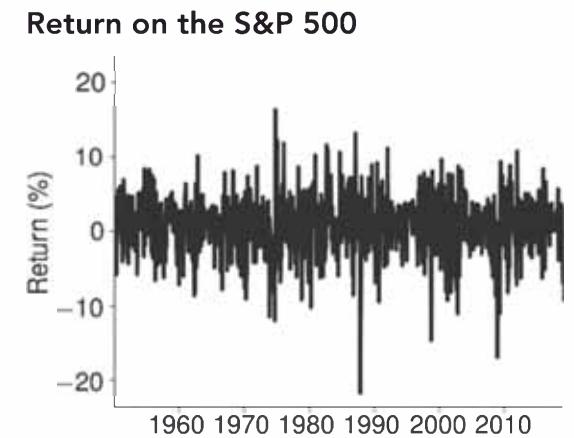
\includegraphics[width=0.50\linewidth]{fig/p34-005.png}
\end{center}
\figcap{A long run of daily returns of the kind POT is applied to. The handful of spikes far
below the mass of observations are the peaks that the threshold is set to isolate.}

% ---------------------------------------------------------
\lo{MR-3 d}{Compare and contrast the generalized extreme value (GEV) and POT approaches to estimating extreme risks.}

Both GEV and POT are rooted in extreme value theory and utilize the tail parameter $\xi$. GEV
focuses on modeling the distribution of extreme values, while POT concentrates on modeling
values exceeding a predefined threshold.

\begin{center}
\small
\begin{tabularx}{\linewidth}{@{}p{2.6cm} >{\raggedright\arraybackslash}X >{\raggedright\arraybackslash}X@{}}
\arrayrulecolor{FRMRule}\toprule
\rowcolor{FRMNavy} \hdr{} & \hdr{GEV} & \hdr{POT}\\
\midrule
\textbf{Models} & The distribution of extreme values (the maxima of large samples).
  & Values exceeding a predefined threshold.\\
\rowcolor{FRMSoft}
\textbf{Shared} & \multicolumn{2}{l}{Both are rooted in extreme value theory and both use the
  tail parameter $\xi$.}\\
\textbf{Parameters} & Often involves estimating an \textit{additional} parameter compared to
  POT, which may result in the loss of useful data.
  & Generally requires fewer parameters.\\
\rowcolor{FRMSoft}
\textbf{Judgement call} & ---
  & Requires selecting a threshold, a decision that can introduce additional uncertainty.\\
\bottomrule
\end{tabularx}
\end{center}

\begin{mrkeybox}
The choice between GEV and POT can be influenced by the nature of the data and specific research
objectives.
\end{mrkeybox}

% ---------------------------------------------------------
\lo{MR-3 e}{Discuss the application of the generalized Pareto (GP) distribution in the POT approach.}

The GP distribution is a type of probability distribution that is commonly used to model extreme
events or excess losses. The Gnedenko-Pickands-Balkema-deHaan (GPBdH) theorem says that as $u$
gets large, the distribution $F_u(x)$ converges to a generalized Pareto (GP) distribution, such
that:

\begin{mrfmlbox}
\begin{align*}
&1 - \left[ 1 + \frac{\xi x}{\beta} \right]^{-1/\xi} && \text{if } \xi \neq 0\\[4pt]
&1 - \exp\!\left[ -\frac{x}{\beta} \right] && \text{if } \xi = 0
\end{align*}
\mrvk{$\xi$ = the tail (or shape) index parameter, the same as it is in GEV theory;\quad
$\beta$ = the scale parameter;\quad $x$ = the excess loss over the threshold.}{}
\end{mrfmlbox}

\begin{enumerate}
\item \term{Shape of the GP distribution.} The GP distribution has a shape that deviates from
      the normal distribution. It initially dips \textit{below} the normal distribution before
      the tail, then rises \textit{above} the normal distribution until it reaches the extreme
      tail. This shape allows the GP distribution to better approximate the behavior of extreme
      events observed in empirical data.
\item \term{Model for excess losses.} The GP distribution is considered a natural choice for
      modeling excess losses because it is based on extreme value theory.
\item \term{Selection of threshold.} Choosing the threshold involves a tradeoff. It needs to be
      \textit{high enough} so the GPBdH theory can apply, but it must be \textit{low enough} so
      that there will be enough observations to apply estimation techniques to the parameters.
\end{enumerate}

\begin{center}
\begin{tikzpicture}
\begin{axis}[
  width=10.4cm, height=5.7cm,
  xmin=0, xmax=5, ymin=0, ymax=0.45,
  axis y line=none, axis x line=bottom, axis line style={draw=black!55},
  tick label style={font=\scriptsize}, xtick={\empty},
  legend style={font=\scriptsize\sffamily, draw=FRMRule, fill=white,
    at={(0.5,-0.30)}, anchor=north, legend columns=-1, column sep=10pt},
  clip=false]
\addplot[domain=0:5, samples=200, smooth, black!80, line width=0.9pt]
  {0.39894*exp(-x^2/2)};
\addlegendentry{Normal}
\addplot[domain=0:5, samples=200, smooth, FRMRed, line width=1.0pt, dashed]
  {0.30*exp(-x/0.78)};
\addlegendentry{Generalized Pareto}
\node[anchor=south, font=\scriptsize\sffamily, text=black!65] at (axis cs:1.05,0.24)
  {dips below};
\draw[black!55, -{Stealth[length=3.5pt]}, line width=0.5pt]
  (axis cs:1.05,0.235) -- (axis cs:1.05,0.15);
\node[anchor=south, font=\scriptsize\sffamily, text=black!65] at (axis cs:3.1,0.10)
  {rises above};
\draw[black!55, -{Stealth[length=3.5pt]}, line width=0.5pt]
  (axis cs:3.1,0.098) -- (axis cs:3.1,0.025);
\end{axis}
\end{tikzpicture}
\end{center}
\figcap{The two curves cross twice. Before the tail the GP density sits under the normal, and
through the tail it sits above it, which is exactly the behaviour empirical loss data shows and
the normal distribution misses.}

\begin{mrkeybox}[title={VaR and expected shortfall}]
One of the goals of using the POT approach is to ultimately compute the value at risk (VaR).
From estimates of VaR, we can derive the expected shortfall (a.k.a.\ conditional VaR).
\end{mrkeybox}

% ---------------------------------------------------------
\lo{MR-3 f}{Explain the multivariate EVT for risk management.}

\begin{itemize}
\item Multivariate EVT studies how extreme events in different variables are connected, like the
      impact of a terrorist attack on oil companies and financial assets.
\item Like univariate EVT, its goal is to estimate extreme events, but for multiple variables.
\item The key focus is \term{``tail dependence''}, where one variable's extreme events relate to
      others.
\item Conventional assumptions and covariance matrices are less useful in multivariate EVT.
\item \term{Copulas} are essential for modeling these multivariate extremes, where the limiting
      distribution falls into the EV copula family.
\item Dealing with multiple variables can be challenging, reducing the number of extreme
      observations and increasing the parameters to estimate.
\end{itemize}

% ==========================================================
